% IEEE conference manuscript; compile from paper/: pdflatex paper.tex (twice).
% Based on the supplied IEEE conference template dated 27 June 2024.
% IEEEtran.cls is an unmodified copy of the supplied class.
% Generated tables are inputs, not hand-transcribed numbers.
\documentclass[conference]{IEEEtran}
\usepackage{cite}
\usepackage{amsmath,amssymb,amsfonts}
\usepackage{booktabs,graphicx}
\usepackage{balance}
\usepackage[hidelinks]{hyperref}
\urlstyle{same}
% Generated from pinned metric files; do not edit.
\newcommand{\CZeroF}{0.2572}
\newcommand{\CZeroM}{0.1024}
\newcommand{\COneF}{0.7533}
\newcommand{\COneM}{0.6779}
\newcommand{\CTwoF}{0.2542}
\newcommand{\CTwoM}{0.0539}
\newcommand{\CThreeF}{0.2728}
\newcommand{\CThreeM}{0.0770}
\newcommand{\CFourF}{0.4208}
\newcommand{\CFourM}{0.2632}
\newcommand{\CFiveF}{0.7288}
\newcommand{\CFiveM}{0.6433}
\newcommand{\CSixF}{0.4688}
\newcommand{\CSixM}{0.1627}
\newcommand{\COneU}{0.7031}
\newcommand{\CTwoU}{0.6674}
\newcommand{\CThreeU}{0.7057}
\newcommand{\CFourU}{0.6687}
\newcommand{\CFiveU}{0.7244}
\newcommand{\CSixU}{0.6865}
\newcommand{\CZeroU}{0.6934}

\title{A Seven-Condition Study of Negative Selection and Hidden Clones in Java Clone Detection}

% Six intentionally blank author/affiliation slots, ordered left-to-right,
% then top-to-bottom, as in the IEEE template. For each contributor, replace
% each complete \phantom{...} expression with that person's actual details.
\author{%
  % Contributor 1
  \IEEEauthorblockN{\phantom{Given Name Surname}}
  \IEEEauthorblockA{\phantom{\textit{Department of Computer Science}}\\
    \phantom{\textit{Name of Institution}}\\
    \phantom{City, Country}\\
    \phantom{email@institution.edu}}
  \and
  % Contributor 2
  \IEEEauthorblockN{\phantom{Given Name Surname}}
  \IEEEauthorblockA{\phantom{\textit{Department of Computer Science}}\\
    \phantom{\textit{Name of Institution}}\\
    \phantom{City, Country}\\
    \phantom{email@institution.edu}}
  \and
  % Contributor 3
  \IEEEauthorblockN{\phantom{Given Name Surname}}
  \IEEEauthorblockA{\phantom{\textit{Department of Computer Science}}\\
    \phantom{\textit{Name of Institution}}\\
    \phantom{City, Country}\\
    \phantom{email@institution.edu}}
  \and
  % Contributor 4
  \IEEEauthorblockN{\phantom{Given Name Surname}}
  \IEEEauthorblockA{\phantom{\textit{Department of Computer Science}}\\
    \phantom{\textit{Name of Institution}}\\
    \phantom{City, Country}\\
    \phantom{email@institution.edu}}
  \and
  % Contributor 5
  \IEEEauthorblockN{\phantom{Given Name Surname}}
  \IEEEauthorblockA{\phantom{\textit{Department of Computer Science}}\\
    \phantom{\textit{Name of Institution}}\\
    \phantom{City, Country}\\
    \phantom{email@institution.edu}}
  \and
  % Contributor 6
  \IEEEauthorblockN{\phantom{Given Name Surname}}
  \IEEEauthorblockA{\phantom{\textit{Department of Computer Science}}\\
    \phantom{\textit{Name of Institution}}\\
    \phantom{City, Country}\\
    \phantom{email@institution.edu}}
}
\begin{document}
\maketitle
\begin{abstract}
We compare random, lexical and semantic negatives, with and without a
token-overlap filter, using a fixed mean-pooled GraphCodeBERT encoder and triplet
objective. The primary benchmark comparison uses three training seeds and a
single untuned reference. Random negatives yield F1 \COneF{}, versus
\CTwoF{} and \CThreeF{} for unfiltered lexical and semantic mining. Filtered
variants improve those two means to \CFourF{} and \CSixF{}, but remain below
random training. A separate functionality-held-out experiment yields unseen
F1 \COneU{} for random training, \CFiveU{} for filtered random training and
\CZeroU{} for the untuned reference. New filtered-condition audit rates are
12, 0 and 22 percent, with substantial uncertainty. These agent/AI judgments
are not independently human-validated. We report a reproducible descriptive
comparison, not a causal identification of contamination dose versus similarity.
Threshold saturation is a diagnostic, not proof of all-negative predictions.
\end{abstract}

\begin{IEEEkeywords}
code clone detection, negative sampling, GraphCodeBERT, contrastive learning,
unseen functionality, audit provenance
\end{IEEEkeywords}

\section{Introduction and Scope}
Negative selection determines which code fragments a contrastive learner is
taught to separate. When a mined negative is an unlabelled clone, this training
signal can conflict with the clone-detection objective.
The question is whether negative selection changes Java clone-detection
performance when the encoder, objective and training budget are fixed. This
study does not establish a universal ranking of mining methods, prove semantic
equivalence by executing code, or reproduce every published configuration.

GraphCodeBERT pretrained weights~\cite{graphcodebert} are used as a
\emph{mean-pooled text encoder}, without explicit data-flow graph input.
Training lasts one epoch over at most 32,000 benchmark triples per condition.
Inputs are capped at 512 tokens, truncating long methods. These restrictions,
incomplete labels and possible cross-split fragment overlap limit validity.
Seed variation is not a significance test or an estimate over new datasets.

All audit judgments are agent/AI review. Historical C2/C3 reviews and the new
C4--C6 pass differ in some functional-granularity conventions. The new protocol
was amended after benchmark outcomes were known, although labels were frozen
before scoring the new sheets. There is no independent human replication or
inter-rater agreement estimate. Wilson intervals quantify sampling variation
under a binomial model, not reviewer bias, outcome awareness, or all dependence
between sampled code pairs.

\section{Design and measurement}
\subsection{Data, model and seven conditions}
The CodeXGLUE clone-detection release~\cite{codexglue} used here has 9,126 source
rows and 8,063 unique Java texts. There are 901,028 training pairs, 415,416
validation pairs and 415,416 test pairs. The test split has 56,820 labelled
positives: prevalence $\pi=0.1367786$. Released labels are the benchmark target,
not a guarantee of semantic equivalence.

The encoder is \path{microsoft/graphcodebert-base}, with mean-pooled,
normalised 768-dimensional representations and cosine scoring. A fixed
triplet-margin objective requires anchor--positive similarity to exceed
anchor--negative similarity by 0.10. The benchmark recipe fixes batch size 8,
learning rate $2\times10^{-5}$, one epoch, a 32,000-triple cap and historical T4
fp16 training. Phase 5 verifies and reports on CPU; no new training occurs.
Table~\ref{tab:conditions} identifies the seven conditions.
\begin{table}[t]
\caption{Negative-Selection Conditions}
\label{tab:conditions}
\centering\footnotesize
\begin{tabular}{ll}
\toprule
Condition & Negative selection \\
\midrule
C0 & Untuned encoder; no project fine-tuning \\
C1 & Random \\
C2 & BM25 lexical ranking \\
C3 & Untuned-embedding semantic ranking \\
C4 & BM25 plus bouncer \\
C5 & Random plus bouncer \\
C6 & Semantic ranking plus bouncer \\
\bottomrule
\end{tabular}
\end{table}
Miners exclude the anchor and known positives, but incomplete labels can leave
unlabelled clones. The bouncer rejects candidates with token-set Jaccard
similarity to the \emph{anchor} at least 0.40, then skips the first ten
survivors. Counted padding still respects the Jaccard cut. This is not a
comparison with the positive snippet or a positive-aware relative threshold.
It changes composition and hardness, not contamination alone. Historical
candidate-rejection shares (0.27\% for C5; 13.6\% for C6) have different
denominators from contamination rates and must not be substituted for them.

\subsection{Metrics and seed denominators}
A pair is predicted clone when its cosine is at least the validation-selected
threshold. Selection uses validation; test is scored with that threshold frozen.
\begin{equation}
F_1=\frac{2TP}{2TP+FP+FN}.
\label{eq:f1}
\end{equation}
Here, $TP$, $FP$ and $FN$ are true positives, false positives and false
negatives, respectively.
The repository's metric called MAP@R ranks all pairs in a split, takes $R$ as
the number of positives, and computes
$(1/R)\sum_{k=1}^{R}P(k)\,\mathrm{rel}(k)$.
It is a split-level ranking score, not an average over per-query retrieval tasks.

The primary benchmark uses seeds 13--15 for C1--C6 and C0 once.
Mean $\pm$ sample SD describes training-seed variation. Six-seed results
(13--18) are a separate extension. A threshold is reported as pinned when
$\tau\geq0.999$, with its denominator shown; this convention does not alter
prediction thresholds.

The separate s$'$ corpus has 4,600 pairs across 23 functionalities, supporting
held-out-functionality evaluation motivated by Kitsios et al.~\cite{unseen}.
The project fixes functionality IDs $\{10,13,14\}$ as held out, uses seeds
13--15 for C1--C6, and evaluates one C0 transfer reference. Threshold selection
uses seen validation, never unseen test outcomes. We report
$\Delta=F_{1,\mathrm{seen}}-F_{1,\mathrm{unseen}}$ and the sample SD of the
three per-seed differences. Seen F1 is measured on that threshold-selection
validation slice, not an independent seen test set; the gap has this asymmetry.
Pair construction and prevalence differ from the
benchmark; absolute F1 levels across corpora are not directly comparable.

\section{Results}
\subsection{Primary benchmark}
Table~\ref{tab:benchmark} reports the primary benchmark comparison.
\begin{table*}[t]
\caption{Seeds 13--15; C0 is a single reference without estimated seed variance.
Thresholds are rounded only for display. Predicted + is the fraction of test
pairs predicted clone.}
\label{tab:benchmark}
\centering\small
\begin{tabular}{lrrrrr}
\toprule
Condition & F1 $\pm$ SD & MAP@R & threshold range & pinned & predicted + \\
\midrule
C0 & 0.2572 & 0.1024 & 0.9779--0.9779 & 0/1 & 22.3--22.3\% \\
C1 & 0.7533 $\pm$ 0.0073 & 0.6779 & 0.4357--0.4492 & 0/3 & 14.2--14.5\% \\
C2 & 0.2542 $\pm$ 0.0108 & 0.0539 & 0.8355--1.0000 & 2/3 & 48.1--87.3\% \\
C3 & 0.2728 $\pm$ 0.0136 & 0.0770 & 1.0000--1.0000 & 3/3 & 33.6--42.7\% \\
C4 & 0.4208 $\pm$ 0.0284 & 0.2632 & 0.4965--0.5414 & 0/3 & 19.3--23.4\% \\
C5 & 0.7288 $\pm$ 0.0029 & 0.6433 & 0.3945--0.4314 & 0/3 & 14.5--14.8\% \\
C6 & 0.4688 $\pm$ 0.0278 & 0.1627 & 0.7955--0.8344 & 0/3 & 28.0--34.9\% \\
\bottomrule
\end{tabular}

\end{table*}
C1 is the strongest primary benchmark condition: F1 \COneF{}, MAP@R \COneM{}.
Unfiltered BM25 and semantic training have much lower mean F1
(\CTwoF{}, \CThreeF{}) and ranking scores (\CTwoM{}, \CThreeM{}).
The bouncer raises their mean F1 to \CFourF{} and \CSixF{}, without reaching C1.
Filtered random C5 obtains \CFiveF{}, below C1's primary mean.
These are descriptive comparisons under the fixed recipe.

The class baseline must be stated correctly: predicting every pair negative
gives $F_1=0$, while predicting every pair positive gives
\begin{equation}
F_{1,\mathrm{all+}}=\frac{2\pi}{1+\pi}=0.2406424.
\label{eq:baseline}
\end{equation}
Neither is a ceiling for useful classification. C2/C3 means are near the weak
all-positive reference, but neither is a constant classifier. Saved primary
predictions mark 48.1--87.3\% of pairs positive for C2 and 33.6--42.7\% for C3.
Near-one thresholds therefore do not mean all-negative predictions. Read
saturation alongside score distributions, prediction counts and ranking.

Figure~\ref{fig:confusion-primary} shows the primary mean confusion matrices.
Each seed is first classified using its own saved threshold; we then average
the four cell counts within each condition. Fractional means are pairs per
run, not pooled totals or ensemble decisions. Colours show actual-row shares
on a common scale, while counts retain the benchmark's class imbalance.
Separate full-resolution images are provided for all 37 benchmark model/seed
runs and for each model's primary and six-seed means.
\begin{figure*}[t]
\centering
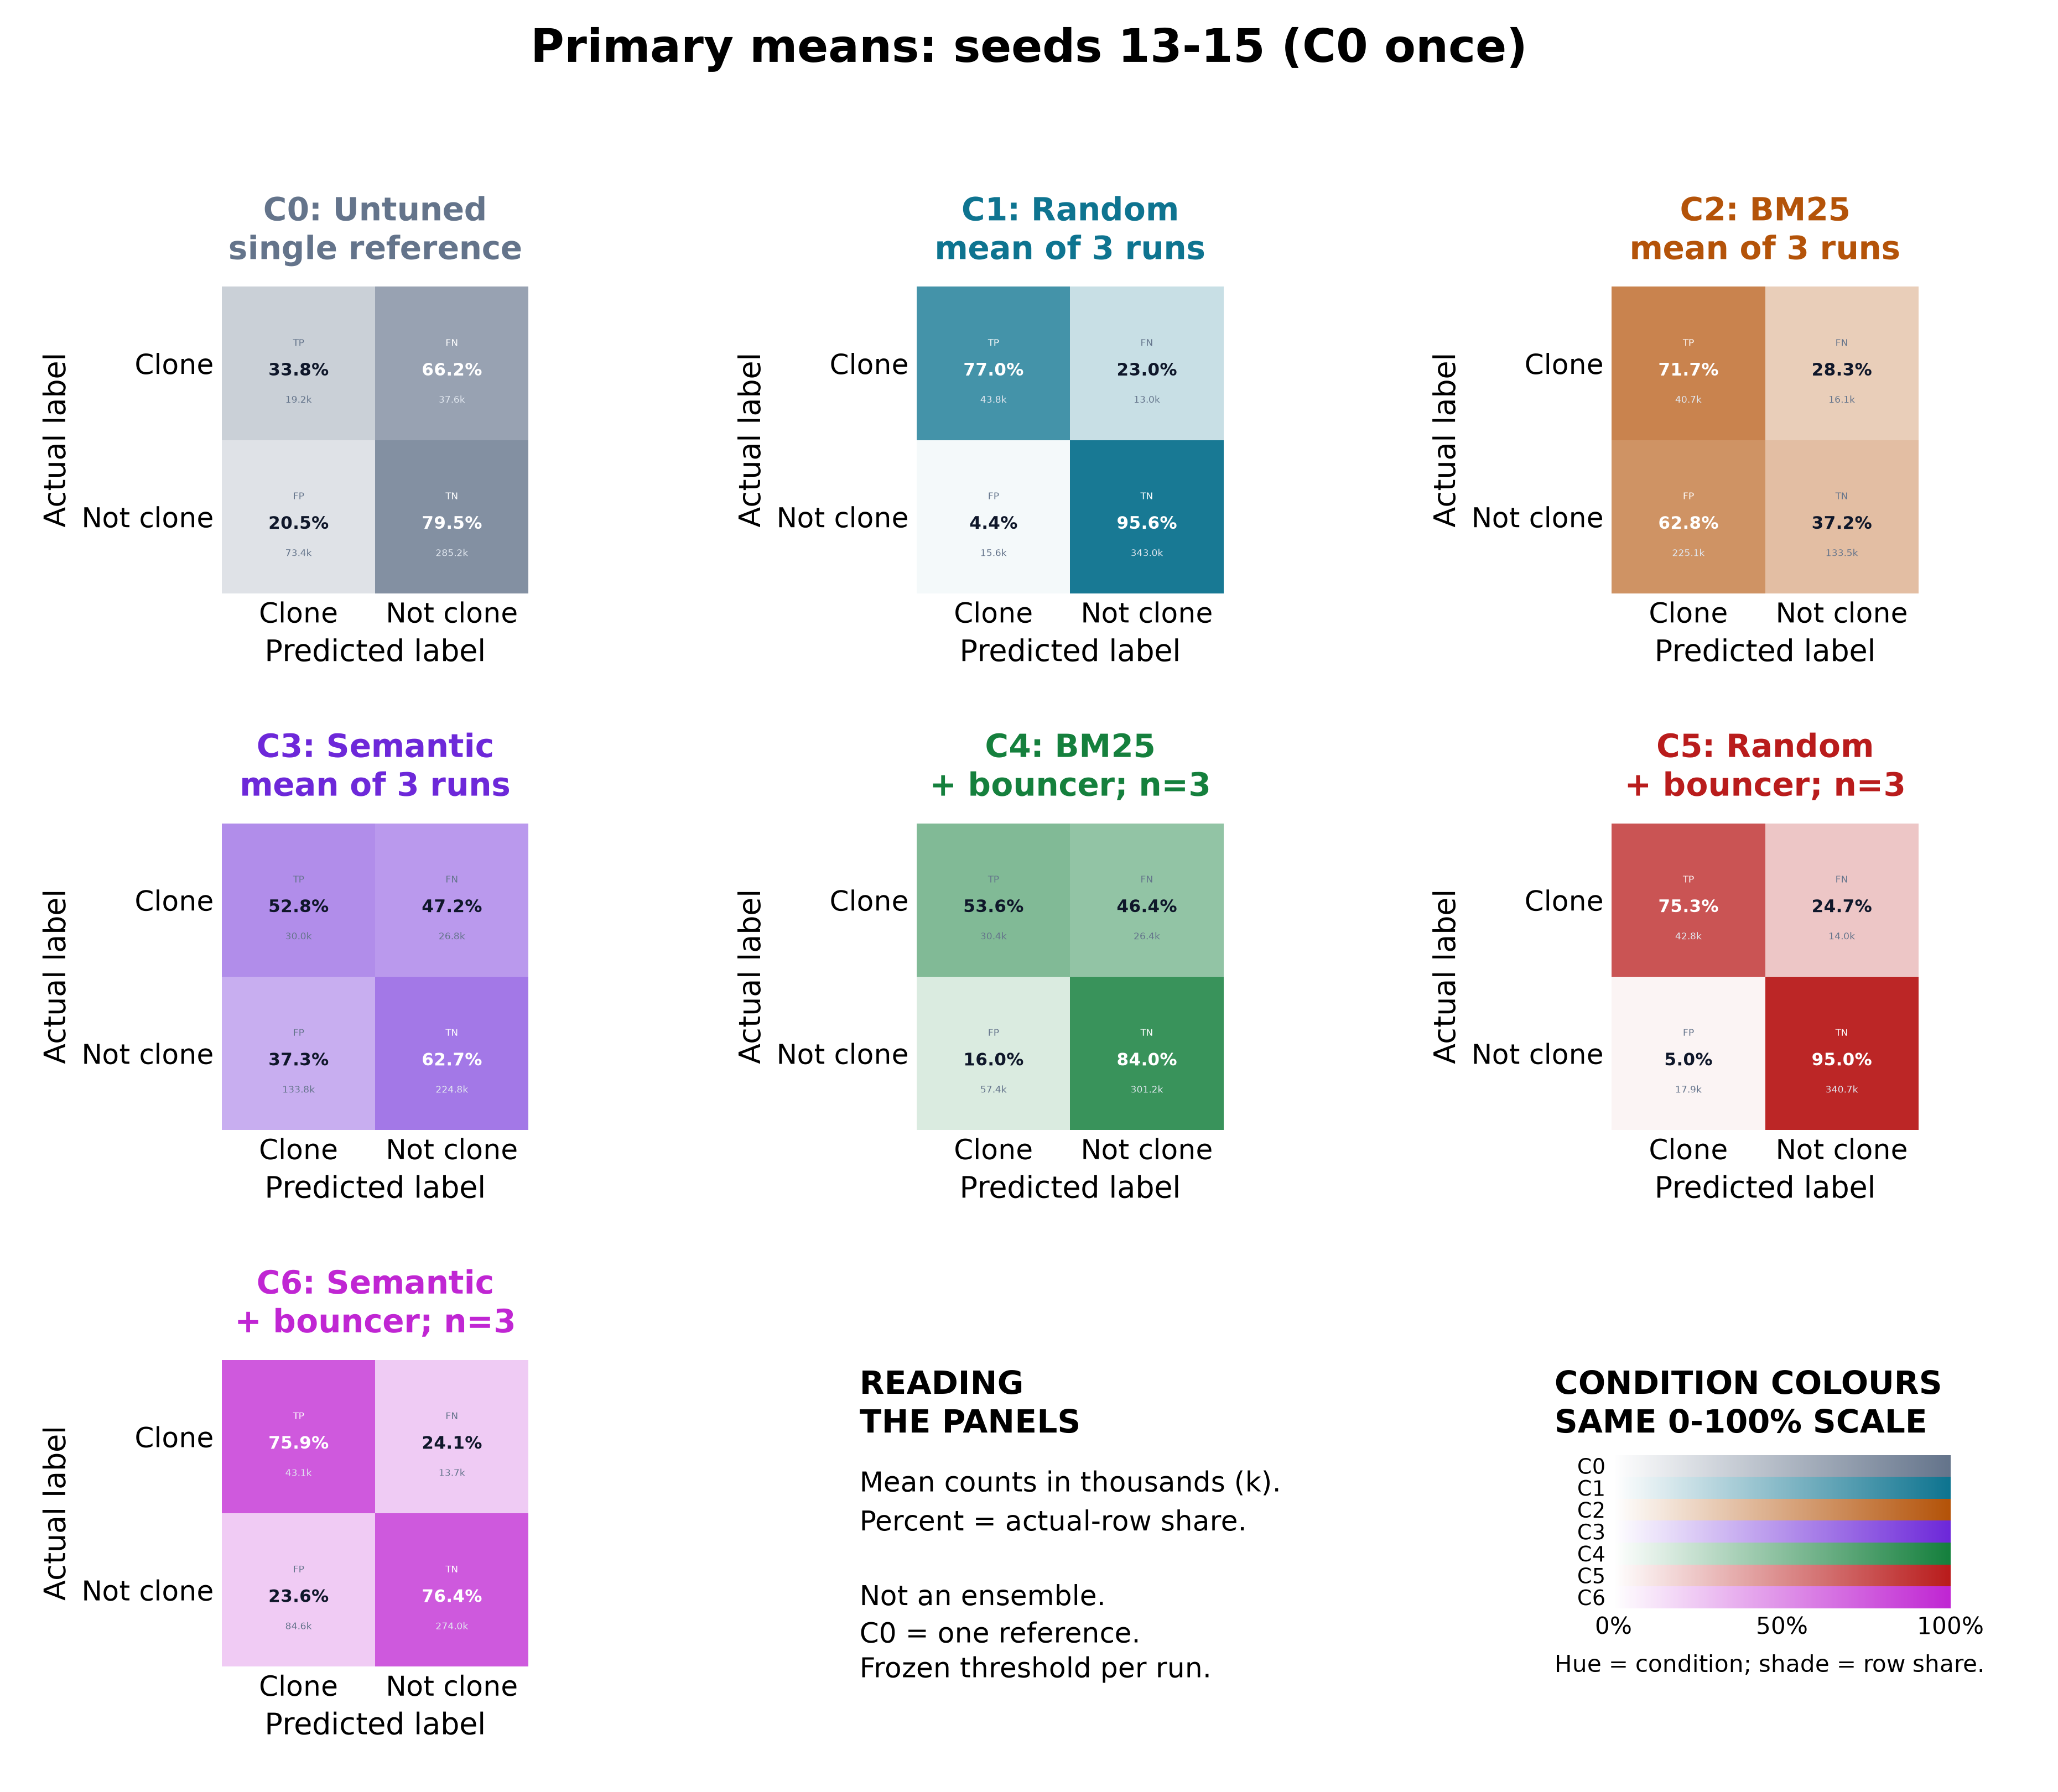
\includegraphics[width=\textwidth]{../report/figures/confusion_matrices/mean_primary_board.png}
\caption{Primary benchmark confusion matrices: C1--C6 are elementwise means
over seeds 13--15; C0 is one untuned reference. Rows are actual labels and
columns are predicted labels, both ordered clone then not-clone, giving
$[[TP,FN],[FP,TN]]$. Counts are mean pairs per run, displayed in thousands
(k); percentages and colour use actual-row normalization. Full counts appear
in the separate per-model images and machine-readable figure record.}
\label{fig:confusion-primary}
\end{figure*}

\subsection{Unseen functionality}
Table~\ref{tab:unseen} reports the separate functionality-held-out experiment.
\begin{table}[t]
\caption{Separate s$'$ experiment, three seeds per trained condition and one
C0 transfer reference. $\Delta$ is seen minus unseen F1, with sample SD of
per-seed differences. A small gap need not indicate a strong classifier.}
\label{tab:unseen}
\centering\footnotesize
\setlength{\tabcolsep}{3pt}
\begin{tabular}{lrrrr}
\toprule
Condition & Seen F1 & Unseen F1 & $\Delta\pm$SD & pinned \\
\midrule
C1 & 0.7570 & 0.7031 & $+0.0539 \pm 0.0222$ & 0/3 \\
C2 & 0.6781 & 0.6674 & $+0.0107 \pm 0.0056$ & 0/3 \\
C3 & 0.7004 & 0.7057 & $-0.0053 \pm 0.0218$ & 3/3 \\
C4 & 0.6731 & 0.6687 & $+0.0044 \pm 0.0055$ & 0/3 \\
C5 & 0.7606 & 0.7244 & $+0.0362 \pm 0.0219$ & 0/3 \\
C6 & 0.7169 & 0.6865 & $+0.0304 \pm 0.0143$ & 0/3 \\
C0 & 0.7118 & 0.6934 & $\text{--}$ & -- \\
\bottomrule
\end{tabular}

\end{table}
C5 has the highest observed unseen mean (\CFiveU{}), followed by C3
(\CThreeU{}) and C1 (\COneU{}); C0 is \CZeroU{}.
The older assertion that no search-mined condition exceeds C0's unseen mean
is false: C3 exceeds it numerically. C3's three thresholds are pinned, requiring
a score-distribution caveat, not a claim of equality with C0. We infer neither
statistical superiority nor equivalence from nearby means.

C2/C4 have small gaps but relatively low absolute unseen F1. C3's negative
mean gap is not itself proof of better generalisation. Benchmark ordering does
not replicate unchanged: C5 and C1 reverse their observed mean ordering.
Report absolute seen/unseen endpoints as well as their difference.

\subsection{Audit evidence}
Table~\ref{tab:audits} gives the audit estimates and their provenance.
\begin{table}[t]
\caption{All labels are agent/AI review, not independently human-validated.
C1 is an estimate, C2/C3 historical reviews, and C4--C6 use amendment
P4-AI-AUDIT-2026-10-23. Incl.\ unsure treats uncertain cases as clones.}
\label{tab:audits}
\centering\footnotesize
\setlength{\tabcolsep}{3pt}
\begin{tabular}{lrrrr}
\toprule
Condition & Clones/$n$ & Rate & Wilson 95\% & Incl. unsure \\
\midrule
C1 & -- & $\approx$0--2\% & -- & -- \\
C2 & 21/50 & 42\% & 29.4--55.8\% & 42\% \\
C3 & 15/50 & 30\% & 19.1--43.8\% & 32\% \\
C4 & 6/50 & 12\% & 5.6--23.8\% & 16\% \\
C5 & 0/50 & 0\% & 0.0--7.1\% & 0\% \\
C6 & 11/50 & 22\% & 12.8--35.2\% & 24\% \\
\bottomrule
\end{tabular}

\end{table}
The new 50-pair sheets contain C4: 6 clone, 42 not-clone, 2 unsure; C5: 0,
50, 0; C6: 11, 38, 1. The point rate is reviewed clones divided by all 50 sampled
training negatives. It estimates hidden-clone contamination under that rubric,
not the classifier's test false-negative rate. Including unsure yields
16\%, 0\% and 24\%.

For $k$ clones in $n$ pairs, let $\hat p=k/n$ and $z=1.96$.
The Wilson interval is $[c-h,c+h]$, where
\begin{equation}
\begin{aligned}
c &= \frac{\hat p+z^2/(2n)}{1+z^2/n},\\
h &= \frac{z\sqrt{\hat p(1-\hat p)/n+z^2/(4n^2)}}{1+z^2/n}.
\end{aligned}
\label{eq:wilson}
\end{equation}
At $0/50$, the upper limit is 7.1\%: C5 is not confirmed contamination-free.
Its point estimate is consistent with the predicted 0--2\% band, but the
population rate is not established to be within it. C4 is below the registered
42\% ceiling, not zero. C6's 22\% point lies below the predicted 25--35\% band
while its interval overlaps it. That audit cannot settle mechanism hypotheses.

\section{Integrity repairs and claim boundaries}
An earlier incident copied C2/C3 labels onto different C4--C6 audit keys.
Those scores were voided; the old C3=C4=30\% premise is withdrawn.
The amended protocol discloses outcome awareness, preserves the blank pack,
freezes labels and pair-specific rationales before key joining/scoring, and
binds scores to hashes. All 150 labels match fixed keys and mining triples;
all 300 displayed fragments match key-indexed canonical code. Freeze time:
23 October 2026, 11:38:33 UTC. Traceability is not independent validity.

A separate repair saves selected thresholds at full precision rather than six
decimals. Nine C2/C3 benchmark runs were re-evaluated; stored test F1 was
unchanged by that repair, while saved prediction thresholds were repaired.
All 37 current benchmark NPZ files replay their recorded F1 within
$5\times10^{-4}$. This is a metric-persistence check, not an independent
reimplementation of the whole experiment.

The confusion-matrix export adds a stricter count comparison. Six runs have
legacy JSON counts different from the frozen NPZ replay. In particular, C3
seed 17 includes 1,780 more true positives and 11,445 more false positives
under its float32 NPZ threshold than under the stored decimal threshold,
although F1 still rounds to 0.2697. The latter comparison reproduces the legacy
counts when performed in float64. Figures use the pinned NPZ scores and
thresholds; source artifacts are unchanged, and all discrepancies are recorded.
F1 agreement alone does not certify precision, recall or count equality.

The evidence supports recipe differences, not a causal isolation of
contamination dose from similarity. The bouncer changes several properties;
review methods differ; the original same-dose comparison was invalid.
A triplet-margin amplifier or special near-duplicate contamination mechanism
remains a hypothesis, not an established result.

Published scores around 0.95 are not reproduced by this mean-pooled adaptation.
Model, training and pair-regime differences are plausible contributors, not a
demonstrated explanation of the entire gap. No test-driven tuning chased that
number. Historical UMAP panels are illustrations, not causal evidence, and
older confusion-board annotations are not reused as repaired predictions here.

\section{Reproducibility and future work}
Inputs are pinned to HF dataset \texttt{Kusshal/Embed}, immutable revision:\\
\texttt{e3144bea7732c20ab2803782282282be4fede7b4}.

The project's guarded CPU notebook performs verification. Its table builder
generates a machine-readable results record containing run identifiers, seed
denominators, prediction-derived positive fractions and 111 input hashes.
Content hashes identify dirty source trees rather than misrepresenting them
as clean releases.

The local HF analysis snapshot omits checkpoints, embeddings and redundant
archives, listing omissions in its manifest; it is not a full model backup.
Local release candidates do not imply Git/HF publication approval.

Independent human replication, a pre-specified denoising ladder and a second
encoder are possible later work, requiring separate protocol/compute decisions.
A parked webpage proposal sends two example Java pairs to C0--C6 on Colab and
shows scores, thresholds and decisions. It is not implemented or experimental
evidence. Example code must never execute; cosine scores are not calibrated
probabilities. No additional compute is allocated for the parked proposal.

\section{Conclusion}
Random negatives outperform unfiltered BM25 and semantic negatives on this
benchmark. Filtering improves those two means but does not reach random
training. Unseen-functionality ordering differs and does not support a blanket
claim that all mined conditions are worse than untuned. Disclosed agent/AI
audits provide uncertain contamination estimates, not human ground truth or
mechanism proof. The deliverable is a provenance-preserving comparison with
correct baselines, exact seed denominators and bounded conclusions.

\appendix[Six-Seed Benchmark Extension]
These are seeds 13--18, not the primary denominator. Historical C3 MAP@R 0.1826
was a transcription error; it belongs to the extension's C6 row.
Table~\ref{tab:extension} keeps these results separate from the primary table.
Figure~\ref{fig:confusion-extension} separately shows the all-seed mean
confusion counts; it does not replace the primary three-seed comparison.
\begin{table}[t]
\caption{Separate Six-Seed Benchmark Extension (Seeds 13--18)}
\label{tab:extension}
\centering\footnotesize
\begin{tabular}{lrrr}
\toprule
Condition & F1 $\pm$ SD & MAP@R & pinned \\
\midrule
C1 & 0.7464 $\pm$ 0.0176 & 0.6674 & 0/6 \\
C2 & 0.2555 $\pm$ 0.0123 & 0.0474 & 4/6 \\
C3 & 0.2733 $\pm$ 0.0091 & 0.0772 & 6/6 \\
C4 & 0.4349 $\pm$ 0.0246 & 0.2760 & 0/6 \\
C5 & 0.7399 $\pm$ 0.0140 & 0.6629 & 0/6 \\
C6 & 0.4722 $\pm$ 0.0282 & 0.1826 & 0/6 \\
\bottomrule
\end{tabular}

\end{table}
\begin{figure*}[t]
\centering
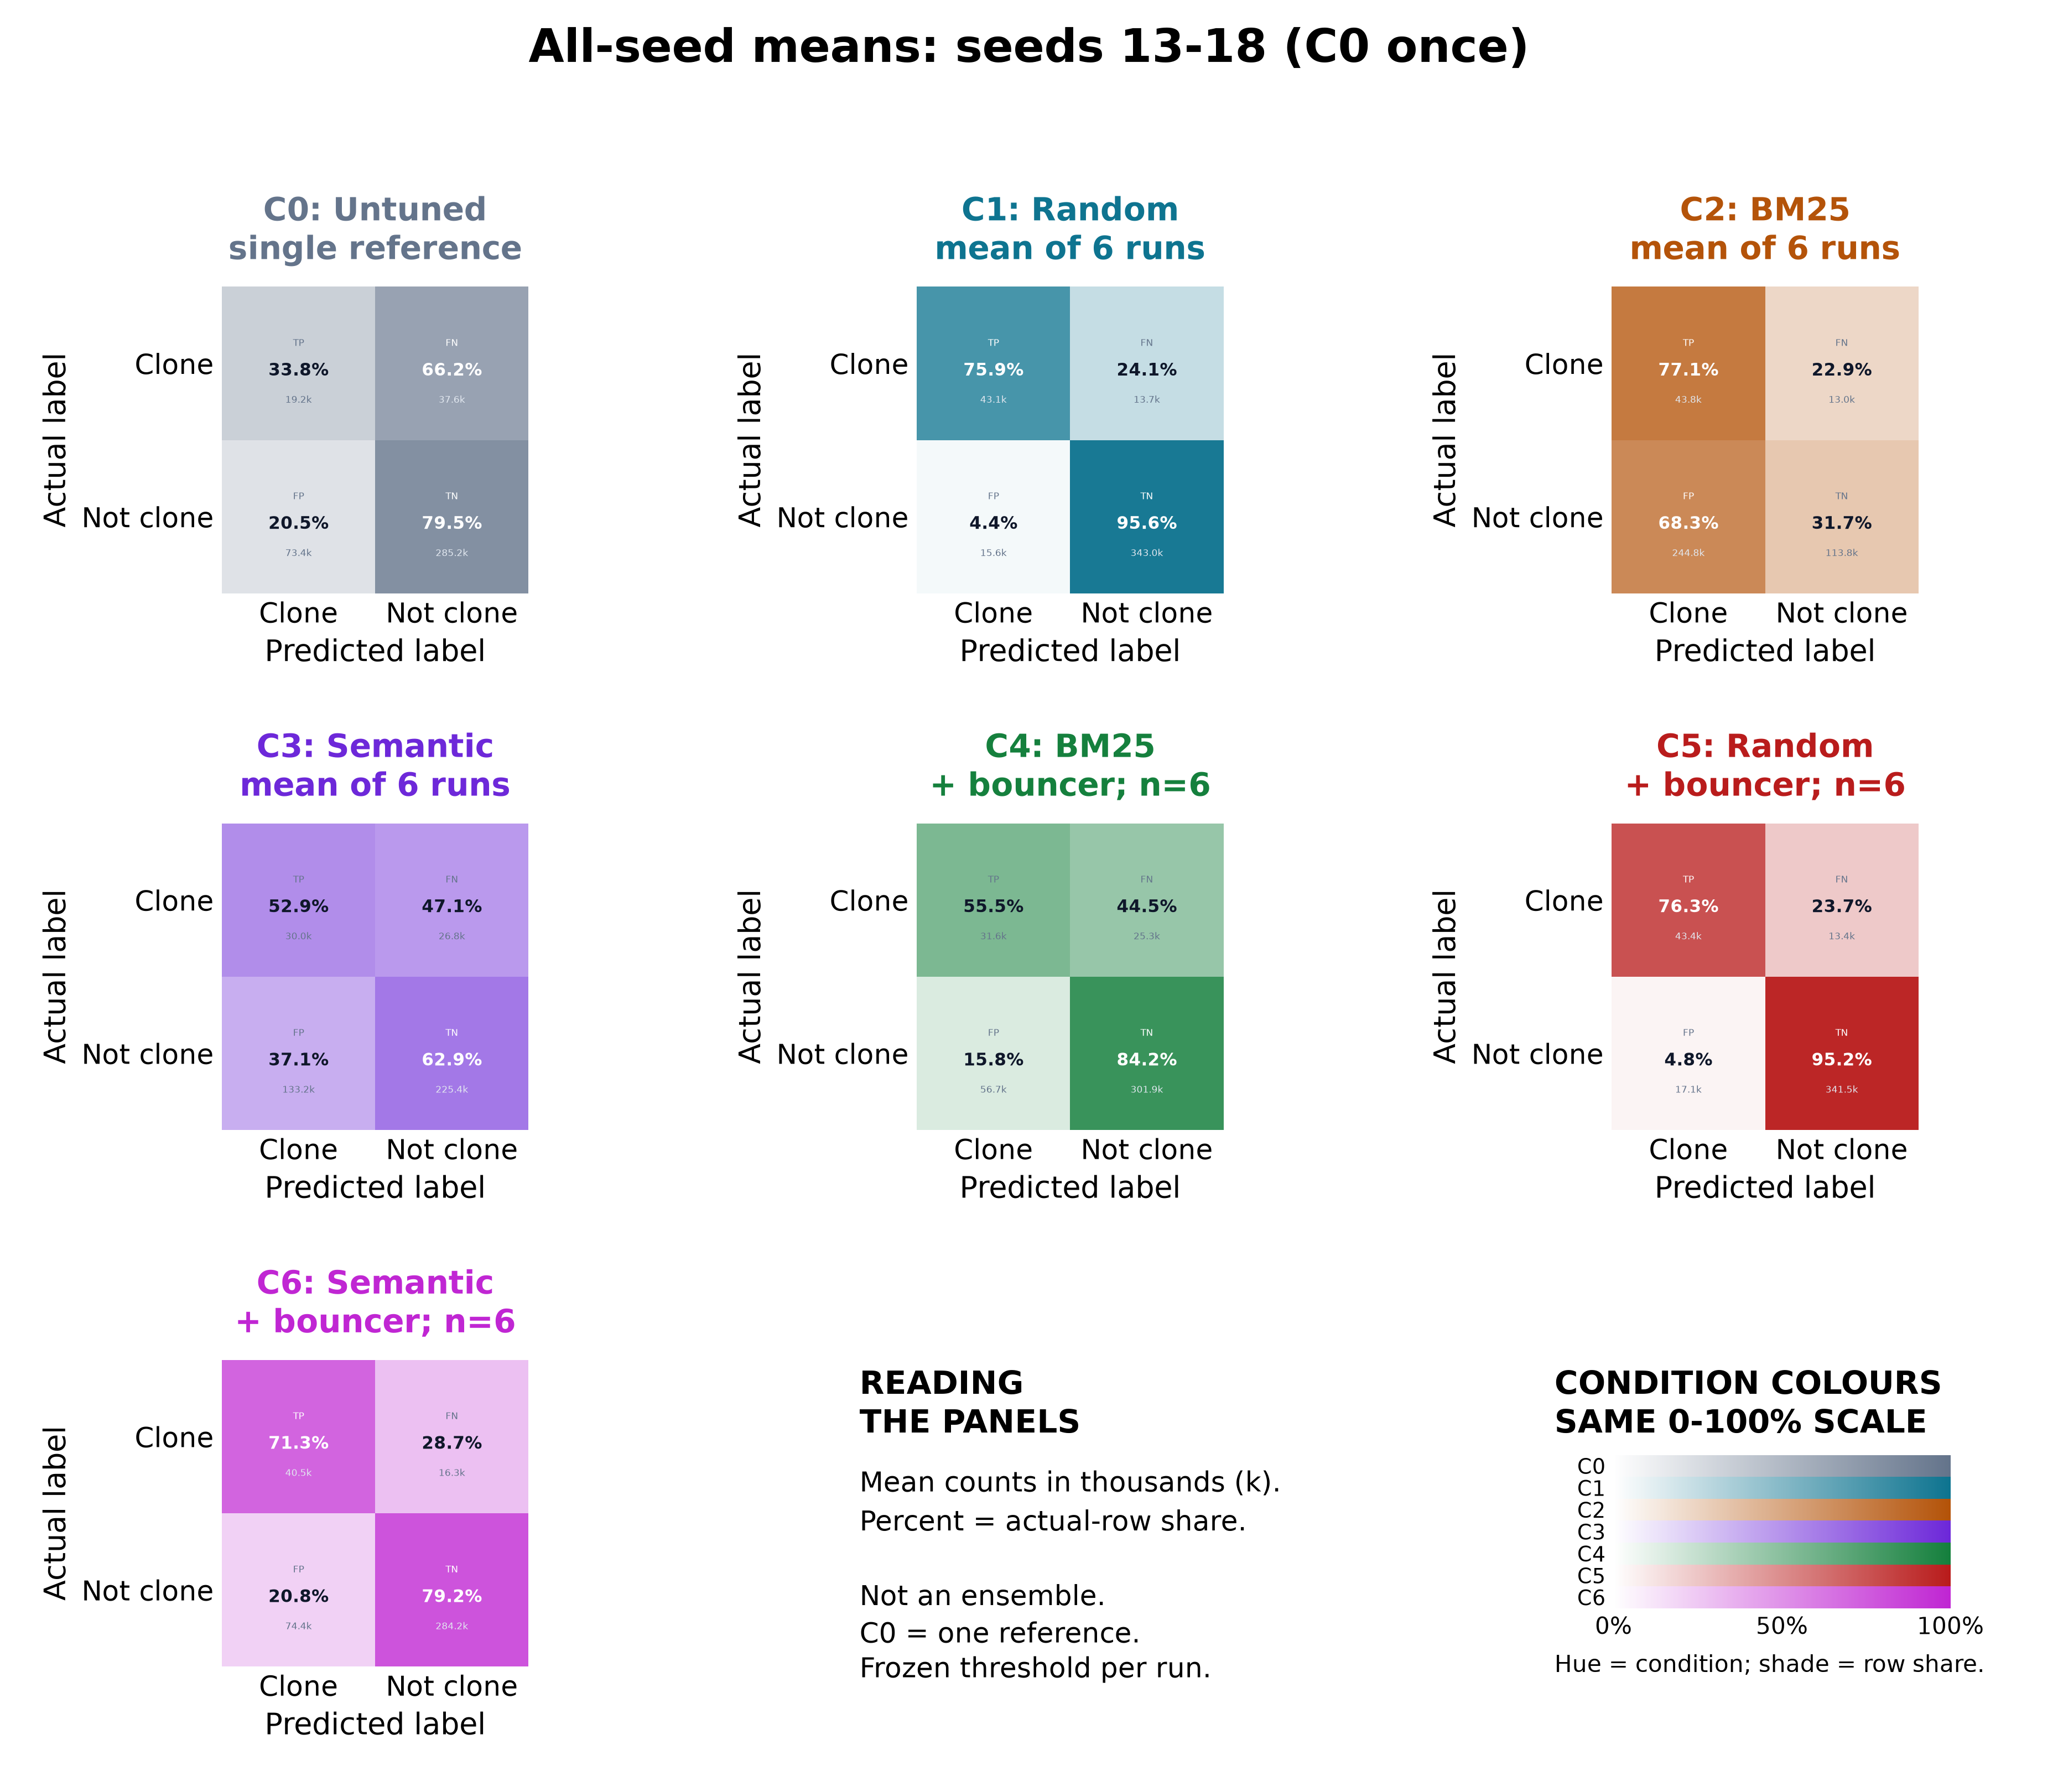
\includegraphics[width=\textwidth]{../report/figures/confusion_matrices/mean_all_seeds_board.png}
\caption{Separate benchmark extension: mean confusion counts over seeds
13--18 for C1--C6, with C0 once. Layout, thousands-of-pairs units and common
actual-row colour scale match Fig.~\ref{fig:confusion-primary}. Each run uses
its own frozen NPZ threshold; no threshold averaging or ensembling is applied.}
\label{fig:confusion-extension}
\end{figure*}

% Start the final appendix-float/reference pair in the first column before
% balancing; revisit this break when the six author blocks are filled.
\newpage
\balance
\begin{thebibliography}{9}
\bibitem{graphcodebert} D. Guo \emph{et al.},
``GraphCodeBERT: Pre-training code representations with data flow,''
in \emph{Proc. Int. Conf. Learn. Represent. (ICLR)}, 2021.
[Online]. Available: \url{https://arxiv.org/abs/2009.08366}
\bibitem{codexglue} S. Lu \emph{et al.},
``CodeXGLUE: A machine learning benchmark dataset for code understanding
and generation,'' 2021, arXiv:2102.04664.
[Online]. Available: \url{https://arxiv.org/abs/2102.04664}
\bibitem{unseen} K. Kitsios, F. Sovrano, E. T. Barr, and A. Bacchelli,
``Detecting semantic clones of unseen functionality,''
in \emph{Proc. IEEE/ACM Int. Conf. Automated Softw. Eng. (ASE)},
2025, doi: \href{https://doi.org/10.1109/ASE63991.2025.00112}{10.1109/ASE63991.2025.00112}.
\end{thebibliography}
\end{document}
